% Latex template: mahmoud.s.fahmy@students.kasralainy.edu.eg
% For more details: https://www.sharelatex.com/learn/Beamer

\documentclass{beamer}					% Document class

\setbeamertemplate{footline}[text line]{%
  \parbox{\linewidth}{\vspace*{-8pt}Differential expression analysis in EndoC-$\beta$H1 beta cells after IFN-$\alpha$ treatment \hfill\insertshortauthor\hfill\insertpagenumber}}
\setbeamertemplate{navigation symbols}{}

\usepackage[english]{babel}				% Set language
\usepackage[utf8x]{inputenc}			% Set encoding

\mode<presentation>						% Set options
{
  \usetheme{default}					% Set theme
  \usecolortheme{default} 				% Set colors
  \usefonttheme{default}  				% Set font theme
  \setbeamertemplate{caption}[numbered]	% Set caption to be numbered
}

% Uncomment this to have the outline at the beginning of each section highlighted.
%\AtBeginSection[]
%{
%  \begin{frame}{Outline}
%    \tableofcontents[currentsection]
%  \end{frame}
\usepackage{graphicx}					% For including figures
\usepackage{booktabs}					% For table rules
\usepackage{hyperref}	
\usepackage{tikz-network}				% For cross-referencing
\usepackage[absolute,overlay]{textpos}
\usepackage{bm}
\usepackage[font=small,labelfont=bf]{caption}				% For cross-referencing

\title{Differential expression analysis in EndoC-$\beta$H1 beta cells after IFN-$\alpha$ treatment}	% Presentation title
\author{Clayton W. Seitz}								% Presentation author
\date{\today}									% Today's date	

\begin{document}

% Title page
% This page includes the informations defined earlier including title, author/s, affiliation/s and the date
\begin{frame}
  \titlepage
\end{frame}


% The following is the most frequently used slide types in beamer
% The slide structure is as follows:
%
%\begin{frame}{<slide-title>}
%	<content>
%\end{frame}

\begin{frame}{Overview}
1. Hybrid microscope setup\\
2. Motivation for studying transcriptional bursting\\
3. Gene selection\\
\end{frame}

\begin{frame}{Widefield-HILO hybrid microscope schematic}


\begin{figure}
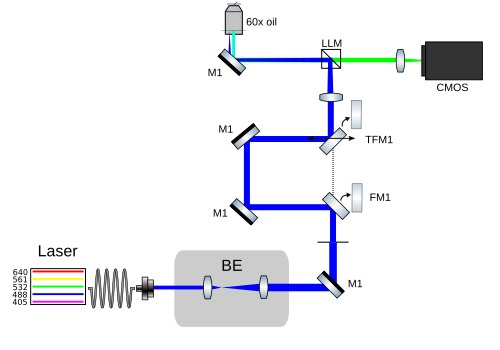
\includegraphics[width=10cm]{epi-hilo.png}
\end{figure}

\end{frame}

\begin{frame}{Example images}

\begin{textblock*}{6cm}(0.25cm,1cm)
\begin{figure}
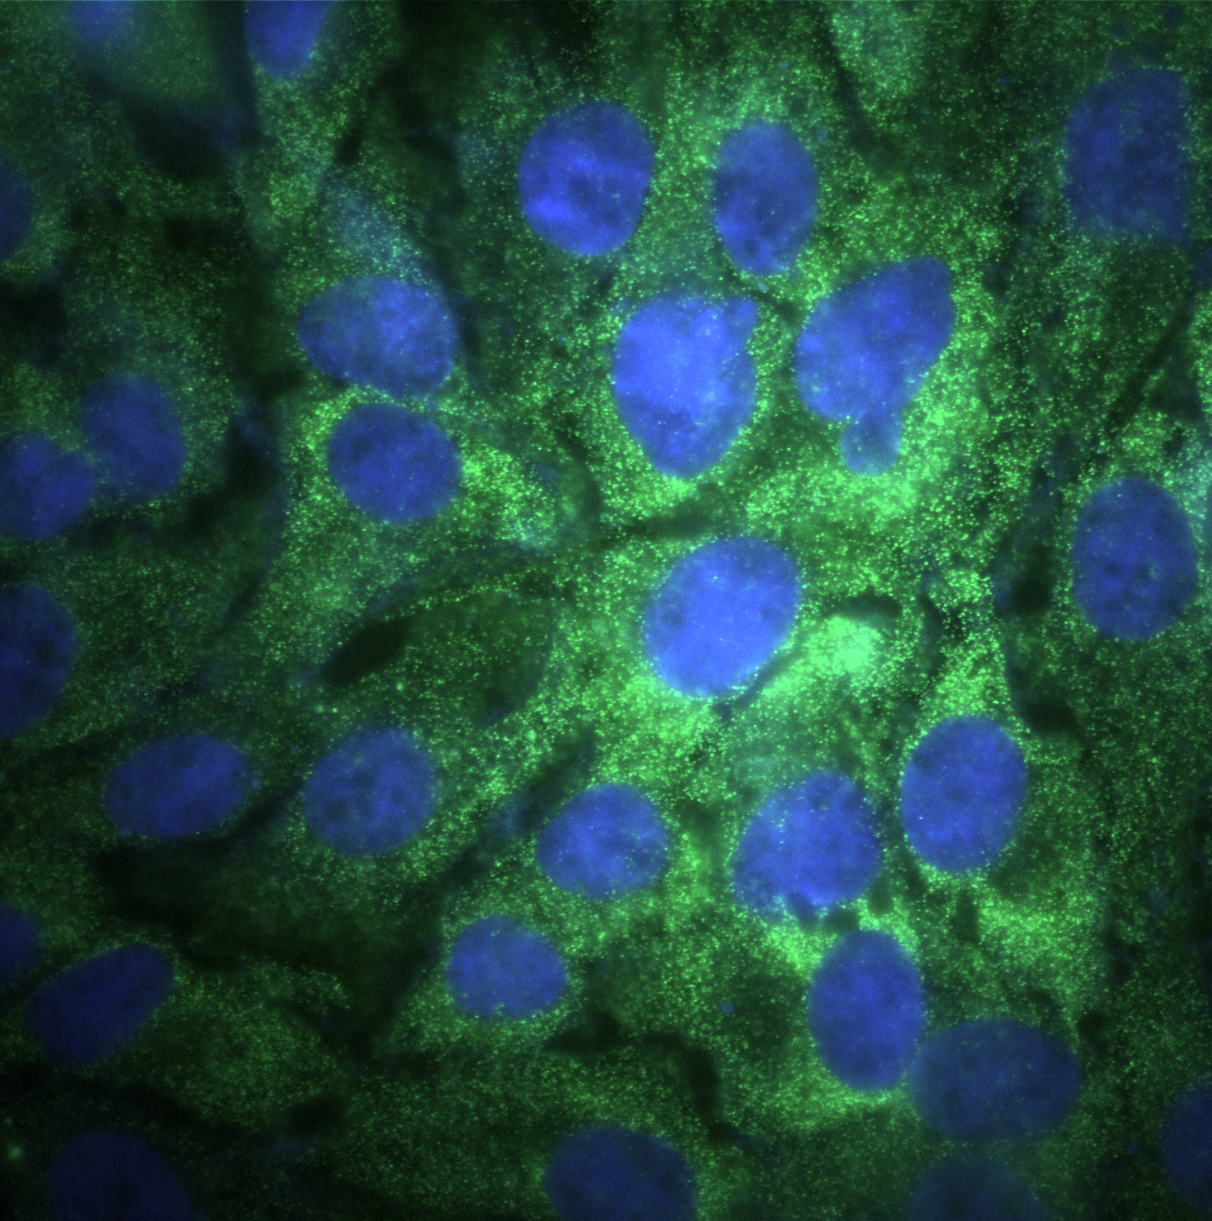
\includegraphics[width=5cm, height=5cm]{dapi-gapdh-1.png}
\end{figure}
\end{textblock*}

\begin{textblock*}{6cm}(6.25cm,1cm)
\begin{figure}
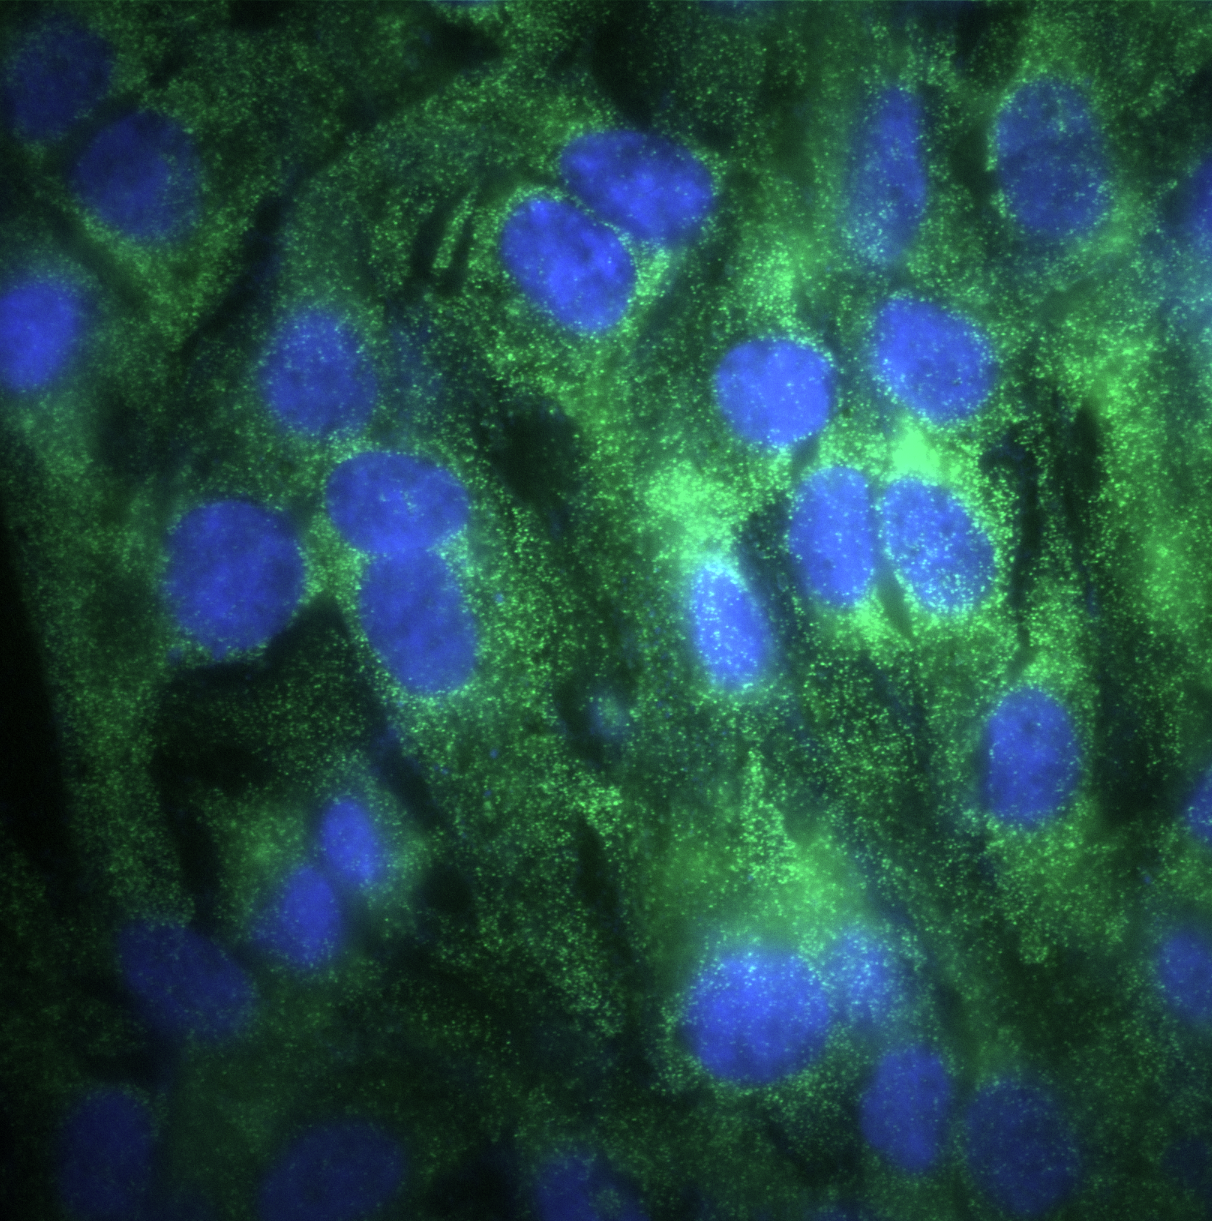
\includegraphics[width=5cm, height=5cm]{dapi-gapdh-2.png}
\end{figure}
\end{textblock*}

\begin{textblock*}{6cm}(0.75cm,1.35cm)
\textcolor{blue}{DAPI}\\
\textcolor{green}{GAPDH}
\end{textblock*}

\begin{textblock*}{15cm}(0.4cm,7cm)
U2OS cells stained for DAPI and human GAPDH (housekeeping gene)\\ using in-situ hybridization\\
\vspace{0.1in}
~100ms and 750ms exposure respectively
\end{textblock*}



\end{frame}


\begin{frame}{Gene expression is stochastic and non-constitutive}


\begin{textblock*}{6cm}(0.25cm,1cm)
\begin{figure}
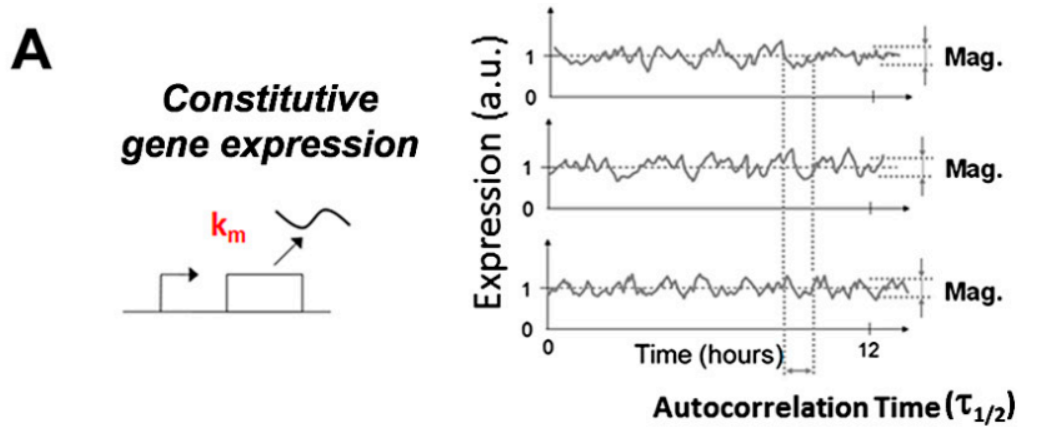
\includegraphics[width=6cm]{burst-1.png}
\end{figure}
\end{textblock*}

\begin{textblock*}{6cm}(6.25cm,1cm)
\begin{figure}
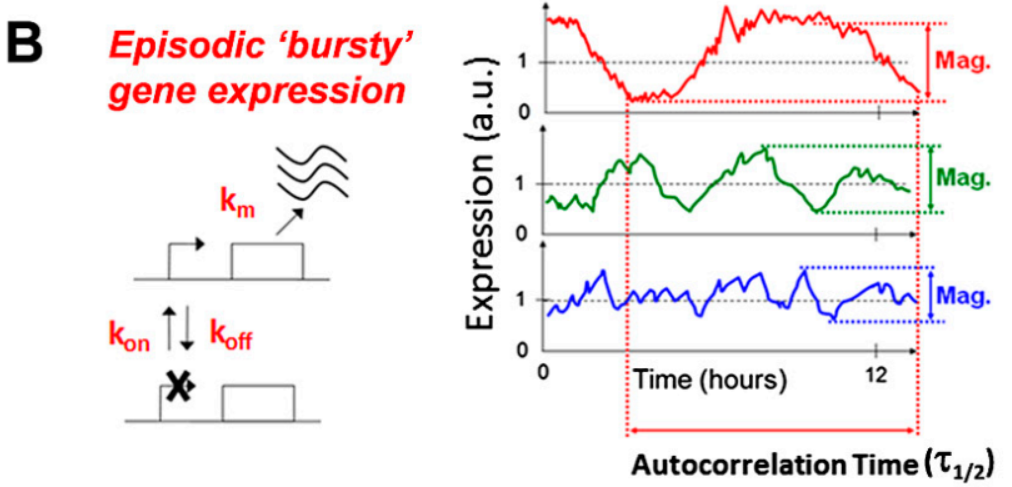
\includegraphics[width=6cm]{burst-2.png}
\end{figure}
\end{textblock*}


\begin{textblock*}{6cm}(0.25cm,5cm)
\hspace{0.5in}\textbf{Single-state models}
\begin{itemize}
\item RNAs are 'born' at a fixed rate
\item RNA counts are Poisson
\end{itemize}
\end{textblock*}

\begin{textblock*}{6cm}(6.25cm,5cm)
\hspace{0.5in}\textbf{Multi-state models}
\begin{itemize}
\item Promoter can be in multiple states
\item RNA counts are not Poissonian
\end{itemize}

\end{textblock*}

\begin{textblock*}{15cm}(0.5cm,8cm)
Single-state models tend to \textcolor{red}{underestimate variance in RNA counts}
\end{textblock*}


\end{frame}

\begin{frame}{EndoC-$\beta$H1 treated with IFN-$\alpha$}

Studies of IFN-$\alpha$ induced expression in cultured cells often lack:
\vspace{0.2in}

\begin{itemize}
\item Single cell resolution of RNA counts and locations
\item Sub-hour time resolution of transcript counts and locations
\item Rigorous statistical models of gene expression
\end{itemize}
\vspace{0.2in}
Starting point:\\
\vspace{0.2in}
Colli, M.L., et al. \textit{An integrated multi-omics approach identifies the landscape of interferon-$\alpha$-mediated responses of human pancreatic beta cells}. Nat Commun 11, 2584 (2020)

\end{frame}

\begin{frame}{Identifying genes: EndoC-$\beta$H1 treated with IFN-$\alpha$}


\begin{figure}
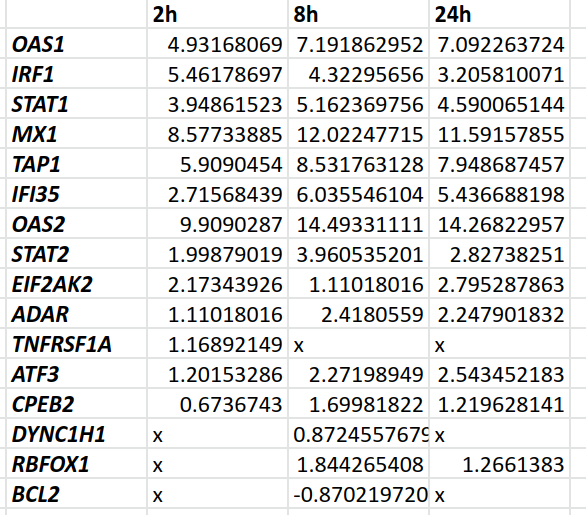
\includegraphics[width=8cm]{fold-change.png}
\end{figure}

\end{frame}

\begin{frame}{Identifying genes: EndoC-$\beta$H1 treated with IFN-$\alpha$ at 2h }


\begin{figure}
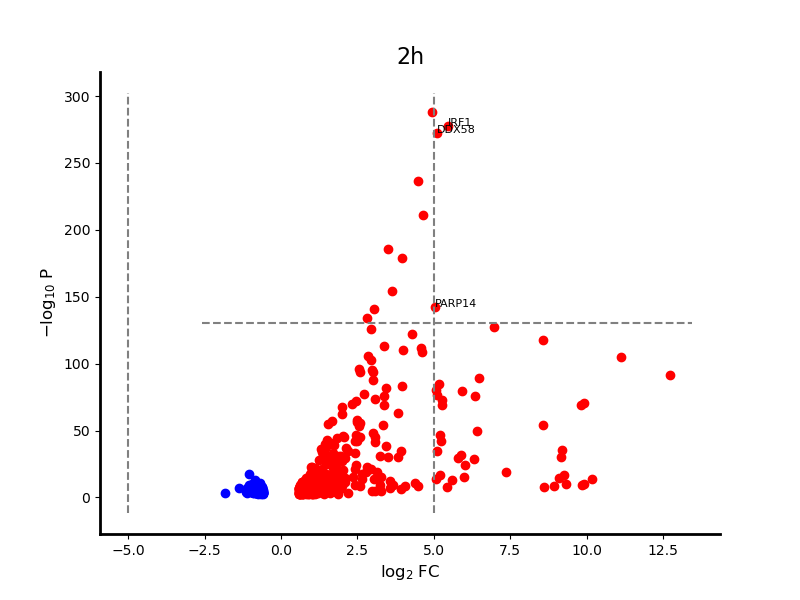
\includegraphics[width=10cm]{volcano-2h.png}
\end{figure}

\end{frame}

\begin{frame}{Identifying genes: EndoC-$\beta$H1 treated with IFN-$\alpha$: 8h }

\begin{figure}
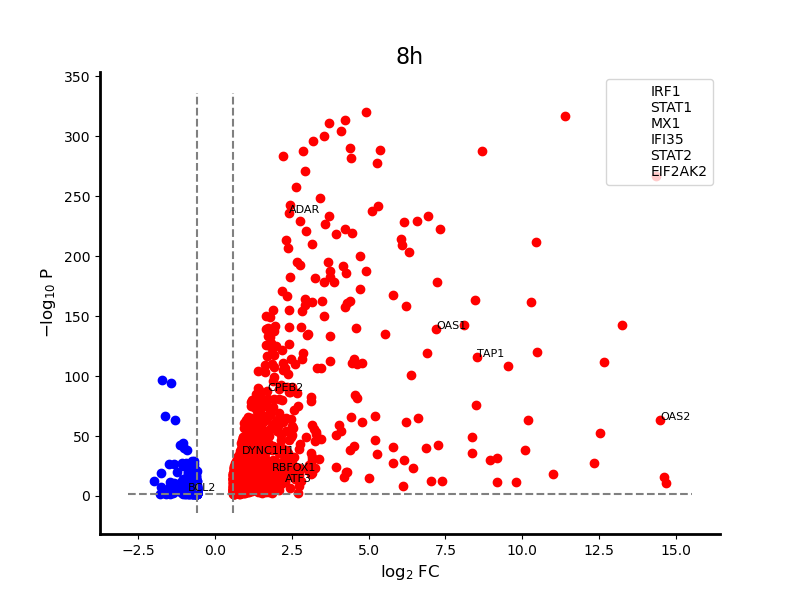
\includegraphics[width=10cm]{volcano-8h.png}
\end{figure}


\end{frame}

\begin{frame}{Identifying genes: EndoC-$\beta$H1 treated with IFN-$\alpha$: 24h }

\begin{figure}
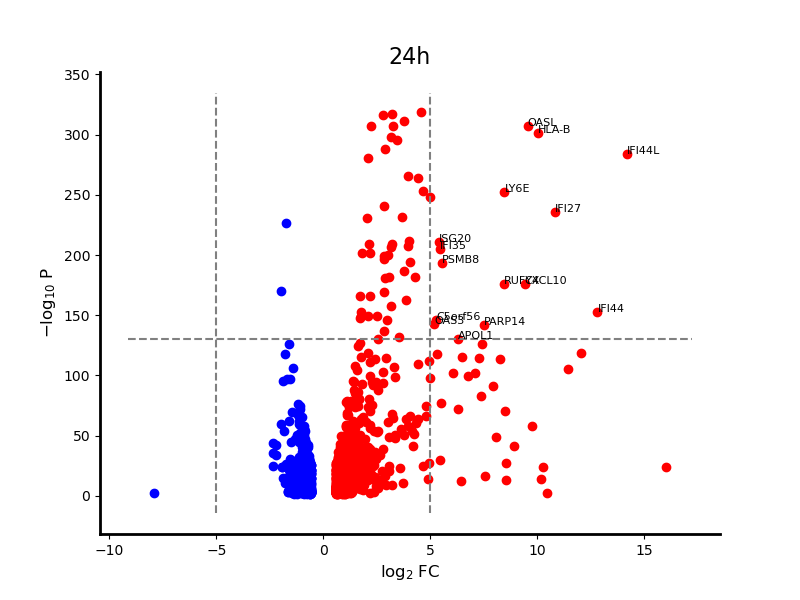
\includegraphics[width=10cm]{volcano-24h.png}
\end{figure}


\end{frame}



\end{document}